\documentclass[tesis]{tesis-usach}

\usepackage[linesnumbered, ruled, vlined, boxed, commentsnumbered, spanish]{algorithm2e}
\usepackage{algpseudocode}
\usepackage{pgfplots}
\usepackage{tikz}
\usepackage{import}
\usetikzlibrary{arrows, calc, decorations.markings, math}
\usetikzlibrary{matrix, chains, positioning, decorations.pathreplacing, shapes, snakes}

\title{Análisis de la eficiencia del entrenamiento de redes neuronales profundas basado en simulated annealing}
\informe{Informe}
\facultad{Facultad de Ingenieria}
\departamento{Departamento de ingenieria informática}

\author{Felipe Alberto Reyes González}
\programa{Magíster en Ingeniería Informática}
\profesor{Victor Parada}
\celular{890 26 317}
\correo{felipe.reyesg@usach.cl}
\date{\today}

\let\cite\shortcite
%\addto\captionsspanish{
%	\renewcommand{\BOthers}[1]{et al.\hbox{}}%
%}

\begin{document}
	\renewcommand{\BOthers}[1]{et al.\hbox{}}%
	\maketitle
	\makecopyright
	\frontmatter
	\indice
	\mainmatter

	%%%%%%%%%%%%%%%%%%%%%%%%%%%%
	% Inicio contenido
	%%%%%%%%%%%%%%%%%%%%%%%%%%%%
	\chapter{Introducción}
\section{Antecedentes y motivación}
Las redes neuronales ({\em Neural Networks}, NN) son sistemas de procesamiento de información que basan su estructura en una analogía de las redes neuronales biológicas. Consisten en un conjunto de elementos de procesamiento simple llamados nodos, estos nodos están dispuestos en una estructura jerarquica y conectadas entre si mediante un valor numérico llamado peso que, mediante un proceso de entrenamiento, varia su valor.

La actividad que una neurona realiza en una NN es simple. El proceso consiste en ponderar las entradas de la neurona por los pesos de las conexiones de la neurona para luego ser sumadas y entregadas a la función de activación asociada a la neurona \cite{McCulloch1943}. La salida corresponderá a la respuesta que la neurona genera a la entrada que se presentada.

El conjunto de $n$ neuronas se llamará capa, y una NN puede estar compuesta de una o más capas. Cada capa estará compuesta por una cantidad de neuronas que no necesariamente será la misma para todas las capas, y estarán dispuesta en forma consecutiva de tal manera que las capas se conecten unas con otras y siempre hacia adelante. La primera capa, la de entrada, recibirá un patrón que será entregado a las distintas neuronas que la capa posea. Cada neurona de la capa de entrada procesará los datos y generará una salida que servirá de entrada para la capa siguiente, repitiendo el proceso para cada una de las capas de la NN hasta llegar a la capa de salida, en cuyo caso la salida representará la respuesta de la red, concretando así el ciclo.

Las NN han sido utilizadas para la clasificación de entradas, y han sido diseñados diversos métodos para entrenar la red y que los pesos se adapten de tal manera que la salida de la red sea representativa de la salida esperada, a esto método de entrenamiento se le llama supervisado.

% https://www.neuraldesigner.com/blog/5_algorithms_to_train_a_neural_network
Dentro de los métodos de entrenamiento existentes se encuentra el método del gradiente descendente, el método de Newton, el gradiente conjugado, el método quasi-Newton, o el algoritmo Levenberg-Marquardt. El más utilizado es el método del gradiente, que consiste en actualizar los pesos de las distintas neuronas en función de la dirección contraría al gradiente de la función de activación, logrando minimizar el error.

%\paragraph{Aprendizaje por corrección del error}: La salida de la NN se compara con la salida esperada, y la diferencia entre ambos valores se utiliza para corregir los pesos de las neuronas. Los pesos de las neuronas se ajustan en función de dicho error hasta ajustarse a los datos que se utilizan para el entrenamiento.

%\paragraph{Aprendizaje estocástico}: Consiste en modificar aleatoriamente los valores de los pesos y observar los resultados para evaluarlos respecto de la salida deseada. Las redes que utilizan este tipo de aprendizaje son una analogía de algún proceso físico basado en estados de energía, donde la red sería el grado de estabilidad y se buscaría el estado de mínima energía, que es el estado donde la respuesta de la red se ajusta de mejor manera a los datos. [37]

\section{Descripción del problema}
%\subsection{El desvanecimiento del gradiente}
La retropropagación basa su funcionamiento en la regla de la cadena para poder calcular los gradientes, y a medida que el error se propaga hacia la capa de entrada de la red él gradiente comienza a disminuír su valor por cada capa que atraviesa. Esto significa que el gradiente disminuirá de manera exponencial, lo que representa un problema para una red de muchas capas, ya que las capas mas cercanas a la capa de entrada necesitarán más tiempo para ser entrenadas.

\section{Solución propuesta}
\subsection{Características de la solución}
Mediante el uso de el algoritmo {\em simulated annealing} se busca analizar la eficiencia que la NN alcanza en una red neuronal profunda frente a otros métodos de aprendizaje.

\subsection{Propósito de la solución}
El propósito de la solución es aportar en el campo de las redes neuronales y la clasificación de datos, proporcionando un análisis comparativo de la convergencia de distintas redes.
\section{Objetivos y alcances del proyecto}
\subsection{Objetivo general}
Evaluar el desempeño del algoritmo {\em simulated annealing} y su efecto sobre entrenamiento de redes neuronales profundas.

\subsection{Objetivos específicos}
Los objetivos establecidos para el presente trabajo son descritos a continuación
\begin{enumerate}
    \item Definir las reglas de aprendizaje a implementar.
    \item Construir los conjuntos de datos de entrada y salida a analizar.
	\item Establecer los parámetros de las redes neuronales para la experimentación.
	\item Entrenar las redes con los distintos conjuntos de datos.
    \item Establecer las conclusiones del trabajo.
\end{enumerate}

\subsection{Alcances}

\section{Metodología y herramientas utilizadas}
\subsection{Metodología de trabajo}
Considerando el aspecto investigativo del trabajo, se considera la utilización del método científico. Entre las actividades que componen la metodología, \citeA{Sampieri2006} describe los siguientes pasos para desarrollar una investigación:

\begin{itemize}
	\item Formulación de la hipótesis: Las redes neuronales que adolecen del desvanecimiento del gradiente se ven beneficiadas por el uso del algoritmo {\em simulated annealing} en la convergencia.

	\item Marco teórico: Una revisión de la literatura donde se aborda el problema planteado, para situarse en el contexto actual de los problemas. Se describirán redes neuronales que buscan solucionar el mismo problema.

	\item Diseño de la solución: Se deberá diseñar el experimento para generar los datos que permitan sustentar las comparaciones entre las distintas redes. Diseñar y ejecutar el experimento basado en entradas equivalentes.

	\item Análisis y verificación de los resultados: Los resultados se analizarán considerando los valores de convergencia de los distintos métodos.

	\item Presentación de los resultados: Se presentarán tablas que describan los resultados obtenidos y que se consideren pertinentes.

	\item Conclusiones obtenidas en el desarrollo de la investigación.
\end{itemize}

\subsection{Herramientas de desarrollo}
Para el desarrollo y ejecución de los experimentos se utilizará un equipo con las siguientes características
\begin{table}[H]
	\centering
	\begin{tabular}{|l|l|}\hline
        Sistema Operativo	& Solus 2017.04.18.0 64-bit\\\hline
        Procesador					& Intel$^\circledR$ Core\texttrademark i5-2450M CPU @ 2.50GHz x 4\\\hline
        RAM								& 7.7Gb\\\hline
		Gráficos				& Intel$^\circledR$ Sandybridge Mobile\\\hline
		Almacenamiento	& 935,6 GB\\\hline
	\end{tabular}
\end{table}

El software que se utilizará es:
\begin{itemize}
	\item Plataforma de desarrollo: Atom.
	\item Lenguaje de programación: Python.
	\item Sistema de redes neuronales: Keras API \cite{Keras2015}.
	\item Herramienta ofimática: \LaTeX.
\end{itemize}

	\chapter{Aspectos teóricos y revisión de la literatura}
\section{Aspectos teóricos}
\subsection{Algoritmo de retropropagación}
Una regla de aprendizaje es el método que le permite adaptar los parámetros de la red. El perceptrón multicapa actualiza sus pesos en función de la salida obtenida de tal manera que los nuevos pesos permitan reducir el error de salida. Por tanto, para cada patrón de entrada a la red es necesario disponer de un patrón de salida deseada.

El objetivo es que la salida de la red sea lo más próxima posible a la salida deseada, debido a esto la es que el aprendizaje de la red se describe como un problema de minimización de la siguiente maner $$ \min_{W} E $$ donde $W$ es el conjunto de parámetros de la red (pesos y umbrales) y $E$ es una función de error que evalúa la diferencia entre las salidas de la red y las salidas deseadas. en la mayor parte de los casos, la función de error se define como:
\begin{eqnarray}
	E = \frac{1}{N}\sum^{N}_{i = 1} e(i)
\end{eqnarray}

Donde $N$ es el número de muestras y $e(n)$ es el error cometido por la red para el patrón $i$, definido de la siguiente manera
\begin{eqnarray}
	e(i) = \frac{1}{n_{C}}\sum^{n_{C}}_{j = 1} (s_{j}(i) - y^{j}(n))^2\label{eq:error_patron}
\end{eqnarray}

Siendo $Y(i) = (y_{1}(i), y_{2}(i), \cdots, y_{n_{C}}(i))$ y $S(i) = (s_{1}(i), s_{2}(i), \cdots, s_{n_{C}}(i))$ los vectores de salida y salidas deseadas para el patrón $i$ respectivamente.

De esta manera, si $W^{*}$ es un mínimo de la función de error $E$, en dicho punto el error será cercano a cero, y en consecuencia, la salida de la red será próxima a la salida deseada.

Así es como el aprendizaje es equivalente a encontrar un mínimo de la función de error. La presencia de funciones de activación no lineales hace que la respuesta de la red sea no lineal respecto a los parámetros ajustables, por lo que el problema de aminimización es un problema no lineal y se hace necesario el uso de técnicas de optización no lineales para su resolución.

Las técnicas utilizadas suelen basarse en la actualización de los parámetros de la red mediante la determinación de una dirección de búsqueda. En el caso de las redes neuronales multicapa, la dirección de búsqueda más utilizada se basa en la dirección contraria del gradiente de la función de error $E$, el método de gradiente descendente.

Si bien el aprendizaje de la red busca minimizar el error total de la red, el procedimiento está basado en métodos del agradiente estocástico, que son una sucesión de minimizaciones del error en función de cada patrón $e(i)$, en lugar de minimizar el error total $E$ de la red. Aplicando el método del gradiente estocástico, cada parámetro $w$ se modifica para cada patrón de entrada $n$ según la siguiente regla de aprendizaje
\begin{eqnarray}
	w(i) = w(n - 1) - \alpha\frac{\partial e(i)}{\partial w}
\end{eqnarray}

donde $e(i)$ es el error para el patrón de entrada $i$ dado por la ecuación \ref{eq:error_patron}, y $\alpha$ es la tasa de aprendizaje, éste último determina el desplazamiento en la superficie del error.

Como las neuronas están ordenadas por capas y en distintos niveles, es posible aplicar el método del gradiente de forma eficiente, resultando en el {\em algoritmo de retropropagación} \cite{Rumelhart1986} o {\em regla delta generalizada}. El término retropropagación es utilizado debido a la forma de implementar el método del gradiente en las redes multicapa, pues el error cometido en la salida de la red es propagado hacia atrás, transformándolo en un error para cada una de las neuronas ocultas de la red.

% Neural Networks for Pattern Recognition - Bishop: 140 - Error backpropagation.
% Neural Networks for Pattern Recognition - Bishop: 263 - Gradient descent.
El algoritmo de retropropagación es el método de entrenamiento más utilizado en redes con conexión hacia adelante. Es un método de aprendizaje supervisado de gradiente descendente, en el que se distinguen claramente dos fases:
\begin{enumerate}
	\item Se aplica un patrón de entrada, el cual se propaga por las distintas capas que componen la red hasta producir la salida de la misma. Esta salida se compara con la salida deseada y se calcula el error cometido por cada neurona de salida.

	\item Estos errores se transmiten desde la capa de salida, hacia todas neuronas de las capas anteriores \cite{Fritsch1996}. Cada neurona recibe un error que es proporcional a su contribución sobre el error total de la red. Basándose en el error recibido, se ajustan los errores de los pesos sinápticos de cada neurona.
\end{enumerate}

\subsection{Problema desl desvanecimiento del gradiente}
El problema del gradiente desvaneciente nace en las NN profundas, éstas utilizan funciones cuyo gradiente tienden a estar entre 0 y 1. Debido a que estos gradientes pequeños se multiplican durante la retropropagación, tienden a {\em desvanecerse} a través de las capas, evitando que la red aprenda en redes muy profundas.

%%%% VER QUE LA NOTACIÓN SEA COMPATIBLE
Si se tiene una NN, la activación de una neurona de una capa intermedia $i$ con función de activación $f_i$ y con entrada $$ net_{i}(t) = \sum_{j}w_{ij}y^{j}(t - 1) $$ es $y^{i}(t) = f_{i}(net_{i}(t))$. Además $w_{ij}$ es el peso de la conexión desde la unidad $j$ hasta la unidad $i$, $d_{k}(t)$ será la respuesta esperada de la unidad $k$ de la capa de salida en el tiempo $t$. Usando el error cuadrático medio ({\em Mean square error}, MSE), el error de $k$ será
$$ E_{k}(t) = (d_{k}(t) - y^{k}(t))^2 $$

En un tiempo $\tau \leq t$ cualquiera, el error de una neurona $j$ que no sea una neurona de entrada es la suma de los errores externos y el error propagado hacia atrás desde la neurona previa será
$$ \vartheta_{j}(\tau) = f'_{j}(net_{j}(\tau))\left(E_{j}(\tau) + \sum_{i} w_{ij}\vartheta_{i}(\tau + 1)\right) $$

El peso actualizado en el tiempo $\tau$ resulta
$$ w_{jl}^{new} = w_{jl}^{old} + \alpha\vartheta_{j}(\tau) y^{l}(\tau - 1)$$
donde $\alpha$ es la tasa de aprendizaje, y $l$ es una unidad arbitraria conectada a la unidad $j$.

En un tiempo arbitrario $\tau \leq t$, el error de la señal en una unidad $j$, que no sea de entrada, será la suma de los errores externos y la señal propagada anterioremente como muestra la ecuación \ref{eq:propagation_error}.
\begin{eqnarray}
	\vartheta(\tau) &=& f'_{j}(net_{j}(\tau)) \left(E_{j}(\tau) + \sum_{i}w_{ij}\vartheta_{i}(\tau + 1)\right)
	\label{eq:propagation_error}
\end{eqnarray}

Entonces, los pesos actualizados serán $$ w_{jl}^{new} = w_{jl}^{old} + \alpha\vartheta_{j}(\tau)y^{l}(\tau - 1) $$
\begin{comment}
Error en el factor de escala. Véase también las contribuciones anteriroes al análisis del desvanecimiento del gradiente \cite{Hochreiter1997a, Bengio1994, Hochreiter1991}. Propagando el error de una unidad $u$ en el timpo $t$ hacia una unidad $v$ {\Huge for $q$ time steps}, el error escala como muestra la ecuación \ref{eq:scale_error}
\begin{eqnarray}
	\frac{\partial \vartheta_{v}(t - q)}{\partial \vartheta_{u}(t)}
	&=&
	\left\{
	\begin{array}{lr}
		f'_{v}(net_{v}(t - 1))w_{uv}&q=1\\
		\\
		f'_{v}(net_{v}(t - q))\sum^{n}_{l = 1}\frac{\partial \vartheta_{l}(t - q + 1)}{\partial \vartheta_{u}(t)}w_{lv}	&q > 1
	\end{array}
	\right.\label{eq:scale_error}
\end{eqnarray}
\end{comment}

\begin{imagen}
	\scalebox{1.0}{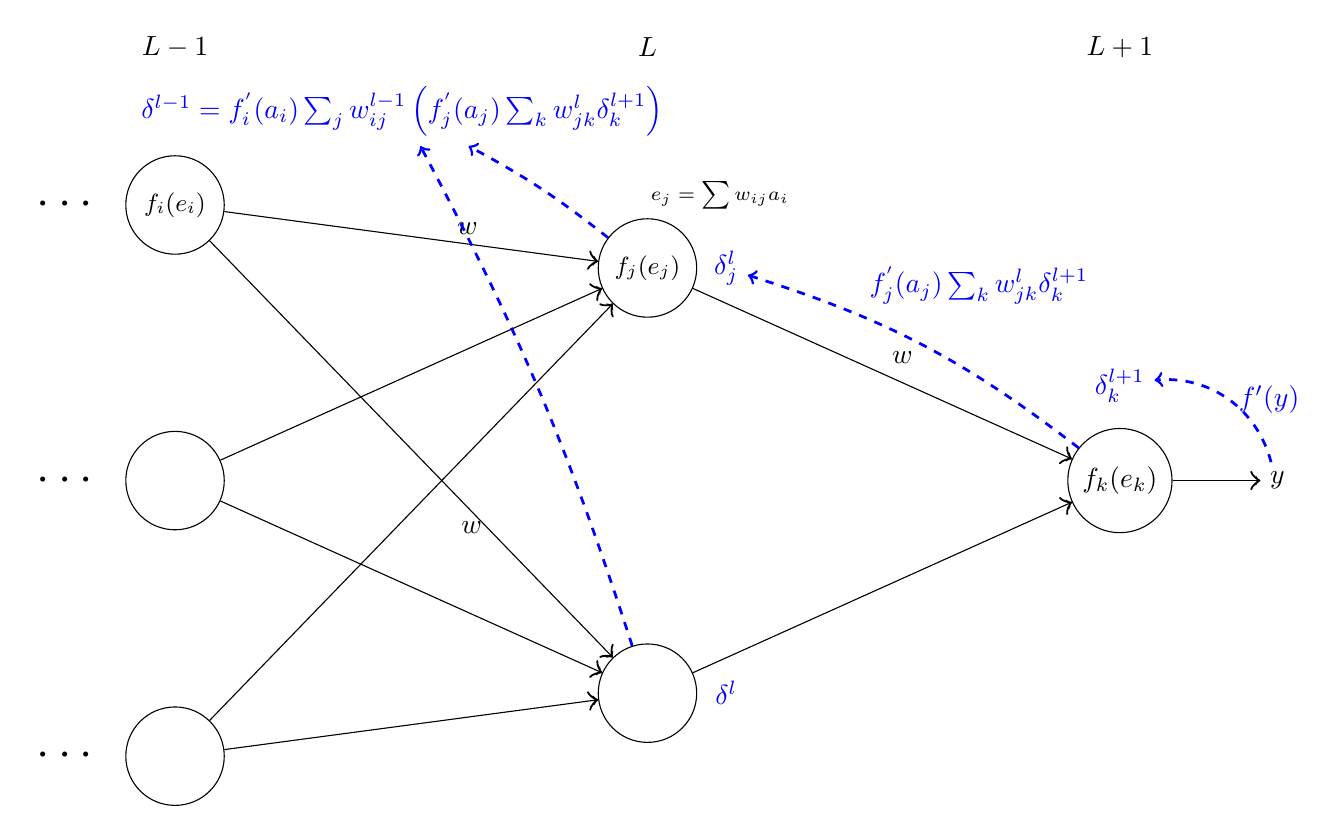
\begin{tikzpicture}

	\tikzstyle{nodo}=[circle, draw, minimum size=1.25cm]
	\tikzstyle{upw}=[dashed, red, ->, line width = 1pt]
	\tikzstyle{cnx}=[->, decoration={markings,mark=at position 1 with {\arrow[scale=2]{>}}}, postaction={decorate},]

	\coordinate (l_0) at (0.0, 5.5);
	\coordinate (l_1) at (6.0, 5.5);
	\coordinate (l_2) at (12, 5.5);

	\coordinate (f_1_1) at (0, 3.5); % CAPA ENTRADA
	\coordinate (f_1_2) at (0, 0); % CAPA ENTRADA
	\coordinate (f_1_3) at (0, -3.5); % CAPA ENTRADA
	\coordinate (f_2_1) at (6.0, 2.7); % CAPA OCULTA 1
	\coordinate (f_2_2) at (6.0, -2.7); % CAPA OCULTA 1
	\coordinate (f_3_1) at (12, 0); % CAPA SALIDA
	\coordinate (y) at (14, 0); % CAPA SALIDA

	\node[] (l_0) at (l_0) {$L - 1$};
	\node[] (l_1) at (l_1) {$L$};
	\node[] (l_2) at (l_2) {$L + 1$};

	\node[nodo, font=\small] (f_1_1) at (f_1_1) {$f_i(e_i)$}; % CAPA ENTRADA
	\node[nodo] (f_1_2) at (f_1_2) {}; % CAPA ENTRADA
	\node[nodo] (f_1_3) at (f_1_3) {}; % CAPA ENTRADA
	\node[nodo, font=\small] (f_2_1) at (f_2_1) {$f_j(e_j)$}; % CAPA OCULTA 1
	\node[nodo] (f_2_2) at (f_2_2) {}; % CAPA OCULTA 1
	\node[nodo] (f_3_1) at (f_3_1) {$f_k(e_k)$}; % CAPA SALIDA
	\node[] (y) at (y) {$y$}; % CAPA SALIDA

	\node[left of=f_1_1, node distance=1.4cm] {\LARGE $\cdots$};
	\node[left of=f_1_2, node distance=1.4cm] {\LARGE $\cdots$};
	\node[left of=f_1_3, node distance=1.4cm] {\LARGE $\cdots$};

	\draw[cnx] (f_1_1) -- node[pos=0.65, above] (w_1_1) {$w$} (f_2_1);
	\draw[cnx] (f_1_2) -- node[pos=0.65, above] (w_1_2) {} (f_2_1);
	\draw[cnx] (f_1_3) -- node[pos=0.65, above] (w_1_3) {} (f_2_1);
	\draw[cnx] (f_1_1) -- node[pos=0.65, below] (w_2_1) {$w$} (f_2_2);
	\draw[cnx] (f_1_2) node[below right of=f_1_2] {} -- node[pos=0.6, below] (w_2_2) {} (f_2_2);
	\draw[cnx] (f_1_3) -- node[pos=0.6, below] (w_2_3) {} (f_2_2);
	\draw[cnx] (f_2_1) node[left of=f_2_1] {} -- node[pos=0.5, above right] (w_j_k) {$w$} (f_3_1);
	\draw[cnx] (f_2_2) -- node[pos=0.5, below right] {} (f_3_1);
	\draw[cnx] (f_3_1) -- node[pos=0.5, below right] {} (y);

	\node[above right of=f_2_1, node distance=1.3cm, font=\scriptsize] {$e_{j} = \sum w_{ij}a_i$};



	\node[blue, above=0.2cm of f_3_1] (e_i) {$\delta^{l+1}_{k}$};
	\node[blue, right of=f_2_1] (e_2_1_i) {$\delta^{l}_{j}$};
	\node[blue, right of=f_2_2] (e_2_2_i) {$\delta^{l}$};
	\node[blue, above right=0.3cm and -1.0cm of f_1_1] (e_1_2_i) {$\delta^{l-1} = f^{'}_{i}(a_i)\sum_{j}w^{l-1}_{ij}\left(f^{'}_{j}(a_{j})\sum_{k}w^{l}_{jk}\delta^{l+1}_{k}\right)$};
	%\node[blue, above right=0.3cm and 0.0cm of f_1_1] (e_1_2_i) {$\delta^{l-1} = f'(a_i)\sum_{j}w^{l-1}_{ij}\delta^{l}_{j}$};

	\draw[upw, blue] (y) to[bend right=40] node[right]{$f'(y)$} (e_i);
	\draw[upw, blue] (f_3_1) to[bend right=10] node[above right, pos=0.7]{$f^{'}_{j}(a_{j})\sum_{k}w^{l}_{jk}\delta^{l+1}_{k}$} (e_2_1_i);
	%\draw[upw, blue] (f_3_1) to[bend left=10] (e_2_2_i);

	\draw[upw, blue] (f_2_1) to[bend right=5] (e_1_2_i);
	\draw[upw, blue] (f_2_2) to[bend right=5] (e_1_2_i);

\end{tikzpicture}
}
	\label{fig:vanishing}
	\caption{Gradiente descendente}
\end{imagen}

\section{Revisión de la literatura}

	%\chapter{Diseño de la experimentación}
\section{Lógica del diseño}

\section{Metodología del experimento}

\section{Consideraciones generales}

	%%%%%%%%%%%%%%%%%%%%%%%%%%%%
	% Fin contenido
	%%%%%%%%%%%%%%%%%%%%%%%%%%%


	%%%%%%%%%%%%%%%%%%%%%%%%
	% Bibliografía
	%%%%%%%%%%%%%%%%%%%%%%%%
	\bibliographystyle{apacite}
	\bibliography{referencias}
	%%%%%%%%%%%%%%%%%%%%%%%%
	% Fin bibliografía
	%%%%%%%%%%%%%%%%%%%%%%%%


	%%%%%%%%%%%%%%%%%%%%%%%%
	% Apéndice
	%%%%%%%%%%%%%%%%%%%%%%%%
	% \appendix
	% \clearpage
	 %\addappheadtotoc
	% \appendixpage
	%%%%%%%%%%%%%%%%%%%%%%%%
	% Fin apéndice
	%%%%%%%%%%%%%%%%%%%%%%%%
\end{document}
